\chapter{Области России}
\label{ch:oblast-of-Russia}
Эта глава книги посвящена исследованию в Викиданных регионов России. 
Отметим, что регионы России включают в себя множество земель разного 
типа: области, республики, края и другие. Именно эти разнотипные регионы 
и были исследованы. Был построен граф субъектов России, граничащих 
с зарубежными странами (граф соседей), а также нарисована карта, 
на которой отмечена численность населения отдельных регионов. Оценка 
степени заполненности свойства Викиданных <<граничит с>> (shares border with) 
показала, что у каждого субъекта РФ эти данные заполнены полностью. 
Читатель познакомится с компьютерной обработкой Викиданных и визуализацией 
информации о регионах России.

\section{Экземпляры объекта <<Области России>>}

Для построения списка всех областей России нам потребуются объект 
\wdqName{<<области России>>}{835714} и свойство \wdProperty{31}{<<экземпляры>>} 
(листинг ~\protect\ref{lst:oblast-of-Russia}).

\begin{lstlisting}[ language=SPARQL, 
                    caption={\href{https://w.wiki/4D2V}{Список всех областей России}\protect\footnotemark},
                    label=lst:oblast-of-Russia,
                    texcl 
                    ]
# List of `instances of` "oblast of Russia"
SELECT ?region ?regionLabel
WHERE
{
    ?region wdt:P31 wd:Q835714. # instance of "oblast of Russia"
    SERVICE wikibase:label { bd:serviceParam wikibase:language "ru"}
}
\end{lstlisting}%
\footnotetext{Получено \num{48} записей в 2017 году и \num{46} записей в 2021 году. Ссылка на SPARQL-запрос: \href{https://w.wiki/4D2V}{https://w.wiki/4D2V}}

В Викиданных больше всего свойств в России и в мире (по данным \href{https://prowd.id/dashboards/68f1cfd5b84d/profile}{ProWD}) у \wdqName{Ленинградской}{2191} и \wdqName{Калининградской областей}{1749}, по 43 свойства. Число свойств для России и мира одинаковое, т.к. и для России и для мира это одни и те же объекты.

Почти пустыми и малоинформативными областями России оказались: \href{http://www.wikidata.org/entity/Q3129}{Орловская область} (\num{31}), \href{http://www.wikidata.org/entity/Q3178}{Курская область} (\num{31}), \href{http://www.wikidata.org/entity/Q5851}{Новосибирская область} (\num{32}).\protect\footnotemark

\footnotetext{По данным ProWD: \href{https://prowd.id/dashboards/68f1cfd5b84d/profile}{https://prowd.id/dashboards/68f1cfd5b84d/profile}}

\section{Субъекты Российской Федерации}

Построим список всех субъектов России~--- республики, края, области, города федерального значения, автономные области и автономные округа (листинг ~\protect\ref{lst:oblast-of-Russia}).

%\footnotetext{
\marginnote{Используемые в SPARQL-запросах объекты:
\begin{itemize}
	\item\wdqName{<<области России>>}{835714};
	\item\wdqName{<<республики России>>}{41162};
	\item\wdqName{<<города федерального значения России>>}{183342};
	\item\wdqName{<<края России>>}{831740};
	\item\wdqName{<<автономные области России>>}{309166};
	\item\wdqName{<<автономные округа России>>}{184122};
	\item\wdqName{<<бывшая административно-территориальная единица>>}{19953632}.
\end{itemize}
Используемые в SPARQL-запросах свойства:
\begin{itemize}
	\item\wdProperty{31}{<<экземпляры>>}
\end{itemize}
}

\begin{lstlisting}[ language=SPARQL, 
                    caption={\href{https://w.wiki/4D2R}{Список всех субъектов России}\protect\footnotemark},
                    label=lst:oblast-of-Russia,
                    texcl 
                    ]
# List of `instances of` "subjects of Russia" 
SELECT ?subject ?subjectLabel ?typeLabel
WHERE
{  
  VALUES ?type {wd:Q835714   # Oblast of Russia
                wd:Q41162    # Republic of Russia
                wd:Q183342   # Federal city of Russia
                wd:Q831740   # Krai of Russia
                wd:Q309166   # Autonomus oblast of Russia
                wd:Q184122}  # Autonomus okrug of Russia
  ?subject wdt:P31 ?type.  # Selecting the type of object
  SERVICE wikibase:label { bd:serviceParam wikibase:language "ru"}
}
\end{lstlisting}%
\footnotetext{Получено \num{85} записей в 2017 году и \num{86} записей в 2021 году. Ссылка на SPARQL-запрос: \href{https://w.wiki/4D2R}{https://w.wiki/4D2R}}

\section{Соседние субъекты}

Построим граф соседних субъектов России по свойству \wdProperty{47}{shares border with} (листинг ~\protect\ref{lst:oblast-of-Russia}).

\begin{lstlisting}[ language=SPARQL, 
                    caption={\href{https://w.wiki/4DKD}{Граф соседних субъектов России}\protect\footnotemark},
                    label=lst:oblast-of-Russia,
                    texcl 
                    ]
# Graph of "subjects of Russia" `shares border with`. 
#defaultView:Graph
SELECT ?sharesBorderWith ?sharesBorderWithLabel ?item ?itemLabel ?rgb
WHERE
{
  VALUES ?toggle { true false }
  
  VALUES ?type {wd:Q835714   # Oblast of Russia
                wd:Q41162    # Republic of Russia
                wd:Q183342   # Federal city of Russia
                wd:Q831740   # Krai of Russia
                wd:Q309166   # Autonomus oblast of Russia
                wd:Q184122}  # Autonomus okrug of Russia
  ?subject wdt:P31 ?type.  # Selecting the type of object  
  
  SERVICE wikibase:label { bd:serviceParam wikibase:language "ru"}
  
  ?subject wdt:P47 ?sharesBorderWith   
           
  BIND(IF(?toggle,?subject, ?type) AS ?item).
  BIND(IF(?toggle,?subjectLabel,?typeLable) AS ?itemLabel).
  BIND(IF(?toggle,"FFFFFF","7FFF00") AS ?rgb).
}
\end{lstlisting}%
\footnotetext{Получено \num{467} записей в 2017 году и \num{480} записей в 2021 году. Ссылка на SPARQL-запрос: \href{https://w.wiki/4DKD}{https://w.wiki/4DKD}}

Полученное число формируется путем сложения количества соседних территорий для всех субъектов России. Результат работы скрипта~--- граф, отображающий соседние субъекты, представлен на рисунке ниже. На нём отчетливо видно изолированную компоненту, которая является Калининградской областью.

\begin{figure*}[h]

    \setlength{\fboxsep}{0pt}%
    \setlength{\fboxrule}{1pt}%
    \fcolorbox{gray}{gray}{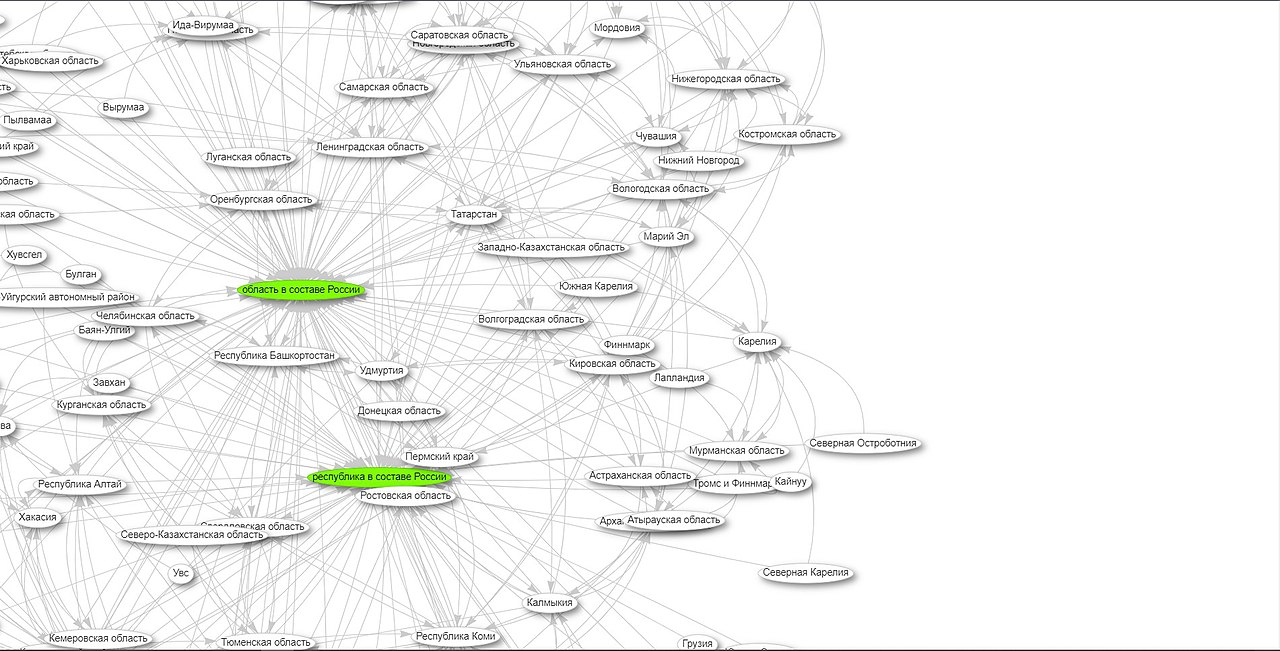
\includegraphics[width=\linewidth]{./chapter/oblast_of_Russia/Graph_Subjects_of_Russia_Karelia.jpg}}
	\caption[Граф субъектов России. Карелия, 2021.]{Граф субъектов России. Карелия, 2021. Граф построен на основе данных, полученных с помощью запроса~\protect\ref{lst:oblast-of-Russia}.}%
\end{figure*} 

\subsection{Полнота Викиданных}

Построим список субъектов России с пустым свойством \wdProperty{47}{shares border with} (граничит с) (листинг ~\protect\ref{lst:oblast-of-Russia}).

\begin{lstlisting}[ language=SPARQL, 
                    caption={\href{https://w.wiki/4DKH}{Список субъектов РФ с пустым свойством \wdProperty{47}{shares border with}}\protect\footnotemark},
                    label=lst:oblast-of-Russia,
                    texcl 
                    ]
# List of "subjects of Russia" without `shares border with`. 
SELECT ?subject ?subjectLabel ?sharesBorderWith ?sharesBorderWithLabel
WHERE
{
  { ?subject wdt:P31 wd:Q835714 } UNION  # Oblast of Russia
  { ?subject wdt:P31 wd:Q41162 } UNION  # Republic of Russia
  { ?subject wdt:P31 wd:Q183342 } UNION  # Federal city of Russia
  { ?subject wdt:P31 wd:Q831740 } UNION  # Krai of Russia
  { ?subject wdt:P31 wd:Q309166 } UNION # Autonomus oblast of Russia
  { ?subject wdt:P31 wd:Q184122 } # Autonomus okrug of Russia
  
  FILTER NOT EXISTS {?subject wdt:P31 wd:Q19953632} # Former administrative territorial entity
  MINUS { ?subject  wdt:P47 [] } . #Shares border with 
  SERVICE wikibase:label { bd:serviceParam wikibase:language "ru"}
}
\end{lstlisting}%
\footnotetext{Получено \num{0} записей в 2017 году и \num{1} записей в 2021 году. Ссылка на SPARQL-запрос: \href{https://w.wiki/4DKH}{https://w.wiki/4DKH}}

С помощью команды FILTER исключаем объекты, которые являются бывшими административно-территориальными единицами. Затем с помощью MINUS отбираем объекты, у которых свойство \wdProperty{47}{<<граничит с>>} незаполнено.

Таким образом, на Викиданных нет изолированных субъектов РФ, что соответствует действительности.

Информация, которая была необходима для решения задачи:
\begin{itemize}
  \item По данным Конституции Российской Федерации Россия состоит из 85 субъектов — республик, краёв, областей, городов федерального значения, автономной области, автономных округов.
  \item В этой задаче не учитываются субъекты, которые на текущий момент времени не входят в состав РФ (например: \wdqName{Читинская область}{182902}), поскольку они не являются экземплярами объектов \wdqName{<<области России>>}{835714}, \wdqName{<<республики России>>}{41162}, \wdqName{<<города федерального значения России>>}{183342}, \wdqName{<<края России>>}{831740}, \wdqName{<<автономные области России>>}{309166}, \wdqName{<<автономные округа России>>}{184122}, а относятся к объекту \wdqName{<<бывшая административно-территориальная единица>>}{19953632}. В этой задаче важно увеличение общего количества субъектов РФ с учётом бывших административно-территориальных единиц увеличится.(Получаем 94 объекта после выполнения SPARQL-запроса. Ссылка на SPARQL-запрос: \href{https://w.wiki/4R2F}{https://w.wiki/4R2F}). 
  \item По данным категории <<Субъекты Российской Федерации>> Русской Википедии существует 85 субъектов РФ.
  \item По данным категории <<\href{https://ru.wikipedia.org/wiki/en:Federal_subjects_of_Russia}{Federal subjects of Russia}>> Английской Википедии так же существует 85 субъектов РФ.
\end{itemize}

\section{Численность населения отдельных субъектов Российской Федерации}

Обозначим на карте субъекты Российской Федерации, разделив их на 6 групп по количеству населения. Субъекты, принадлежащие одной группе, будут отображаться на карте одним цветом, а именно:
\begin{itemize}
  \item субъекты с количеством населения менее \num{500000} обозначаются синим цветом
  \item субъекты с количеством населения более \num{500000}, но менее \num{1000000} обозначаются оранжевым цветом
  \item субъекты с количеством населения более \num{1000000}, но менее \num{3000000} обозначаются зеленым цветом
  \item субъекты с количеством населения более \num{300000}, но менее \num{8000000} обозначаются красным цветом
  \item субъекты с количеством населения более \num{800000}, но менее \num{10000000} найдены не были
  \item субъекты с количеством населения более \num{1000000} обозначаются фиолетовым цветом
\end{itemize}

Для запроса нам потребуются свойства \wdProperty{625}{<<координаты>>} и \wdProperty{1082}{<<численность населения>>}.

\begin{lstlisting}[ language=SPARQL, 
                    caption={\href{https://w.wiki/4DKV}{Карта населения России}\protect\footnotemark},
                    label=lst:oblast-of-Russia,
                    texcl 
                    ]
# Map of `population` "subject of Russia"
# Version 2021
#defaultView:Map
SELECT DISTINCT ?subject ?subjectLabel ?population ?coord ?layer
{
  {
    { ?subject wdt:P31 wd:Q835714 } UNION  # Oblast of Russia
    { ?subject wdt:P31 wd:Q41162 } UNION  # Republic of Russia
    { ?subject wdt:P31 wd:Q183342 } UNION  # Federal city of Russia
    { ?subject wdt:P31 wd:Q831740 } UNION  # Krai of Russia
    { ?subject wdt:P31 wd:Q309166 } UNION # Autonomus oblast of Russia
    { ?subject wdt:P31 wd:Q184122 } # Autonomus okrug of Russia
  }   
  ?subject wdt:P625 ?coord; wdt:P1082 ?population.
  
  FILTER NOT EXISTS {?subject wdt:P31 wd:Q19953632}  # former administrative territorial entity
  BIND(
    IF(?population < 500000, "< 500000",
    IF(?population < 1000000, "500000 - 1000000",
    IF(?population < 3000000, "1000000 - 3000000",
    IF(?population < 8000000, "3000000 - 8000000",
    IF(?population < 10000000, "8000000 - 10000000",
    "> 10000000")))))
    AS ?layer).
  
  SERVICE wikibase:label { bd:serviceParam wikibase:language "ru"}
}
ORDER BY ?population
\end{lstlisting}%
\footnotetext{Получено \num{85} записей в 2017 году и \num{86} записей в 2021 году. Ссылка на SPARQL-запрос: \href{https://w.wiki/4DKV}{https://w.wiki/4DKV}}

Результат работы скрипта (листинг ~\protect\ref{lst:oblast-of-Russia}) представлен на рисунке ниже.

\begin{figure*}[h]

    \setlength{\fboxsep}{0pt}%
    \setlength{\fboxrule}{1pt}%
    \fcolorbox{gray}{gray}{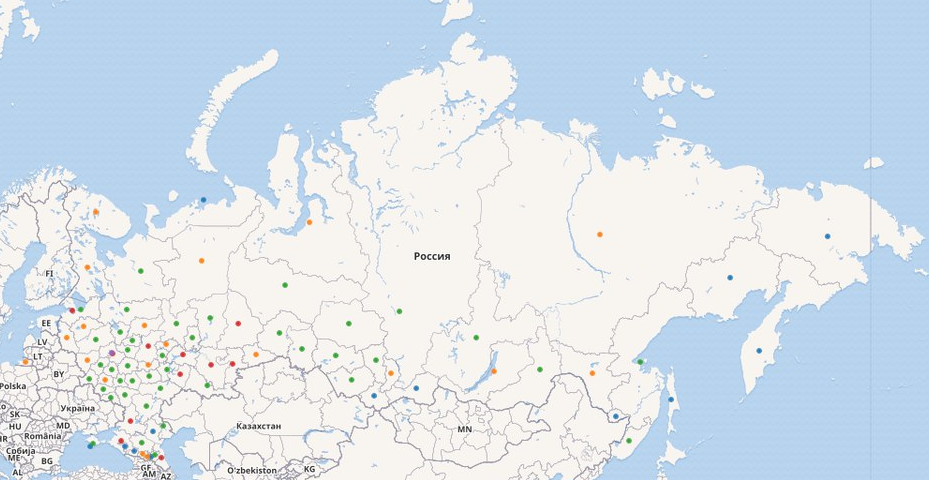
\includegraphics[width=\linewidth]{./chapter/oblast_of_Russia/SubjectsRussia_Map.png}}
	\caption[Карта населения России, 2021.]{Карта населения Российской Федерации, 2021. Карта субъектов Российской Федерации, разделённых на 6 групп по количеству населения и отмеченных разными цветами в зависимости от группы, в которую субъект входит. Карта построена на основе данных, полученных с помощью запроса~\protect\ref{lst:oblast-of-Russia}.}%
\end{figure*} 

\section{Защита страниц}

На страницы Викиданных устанавливается защита для предотвращения повторяющегося вандализма или спама. Существует несколько видов защиты:
\begin{itemize}
  \item Частичная защита или полузащита (обозначается серым замком) разрешает редактировать страницу только автоподтверждённым/подтверждённым участникам.
  \item Полная защита (обозначается оранжевым или красным замком) ограничивает круг редакторов администраторами.
  \item Защита от переименования (обозначается зелёным замком) не ограничивает возможность редактировать страницу, однако переименовать её могут только администраторы. Большинство популярных страниц защищено от переименования. Защита от переименования не может быть применена к страницам элементов или свойств.
  \item Защита от создания (как полная, так и частичная защита обозначается синим замком) может применяться к удалённым или несуществующим страницам. Однако, как и защита от переименования, она не может применяться к удалённым элементам или свойствам.
  \begin{itemize}
	\item При полной защите от создания страницу не может создать никто, кроме администраторов.
	\item При частичной защите от создания страницу могут создать также автоподтверждённые и подтверждённые участники.
  \end{itemize}
\end{itemize}

В крайне редких случаях Фонд Викимедиа может защитить страницу в качестве официального действия (office action, обозначается чёрным замком). Официальные действия совершаются только в результате формальной вневикипедийной жалобы, всегда публично объявляются и выполняются только сотрудниками Фонда Викимедиа или членами Совета попечителей.

Дополнительную ссылку Вы можете найти в справочных страницах Викиданных\protect\footnotemark
\footnotetext{\href{https://www.wikidata.org/w/index.php?title=Wikidata:Protection_policy/ru&oldid=1413630638}{Правила защиты страниц}}.